\section{Flag \& Ball Interaction} \label{flag-interaction}
This section codifies the rules for how the flags and the ball are interacted with.

Flags and balls are picked up automatically when a player enters their hex.

\subsection{The Flag}
The flag is present in each of the teams' capture zones.
The flag can be thrown (see \secref{throwing}) based on a player's \throw{} score (see \secref{the-team}).

\begin{table}[!ht]
    \centering
\begin{tabular}{r|l}
    \textbf{Point Value} & 1 \\
    \textbf{Movement Penalty} & $None$ \\
    \textbf{Can be Thrown?} & Yes \\
    \textbf{Special Note} & Capturing the flag doesn't immediately award points. \\
\end{tabular} 
    \caption{flag Stats}
    \label{tab:flag}
\end{table}
The thrown flag can be intercepted by an opposing player.
To do this, the pass must intersect the opposing player's reach.
The flag is successfully intercepted if the opposing player rolls \blank{} or \plus{} on 1dF.

Every opposing player whose reach it intersects gets an attempt at intercepting the throw (see \secref{interception}).

On a successful interception, roll scatter as if intercepting player was the target of the pass (see \secref{scattering}).

\subsection{The Ball}
The Ball is a special heavy object that resides in the middle of the playing field.
The Ball is impractically heavy, and thus impedes movement, and cannot be thrown.
However, it can be handed off (see \secref{handing-off})

\begin{table}[!ht]
    \centering
\begin{tabular}{r|l}
    \textbf{Point Value} & $0$ \\
    \textbf{Movement Penalty} & $Move\div 2$ \\
    \textbf{Can be Thrown?} & No, but can be handed off \\
    \textbf{Special Note} & Ends a Third the moment it’s captured.\\
\end{tabular}
    \caption{Heavy Stats}
    \label{tab:heavy}
\end{table}
You only receive points for flags in your capture zone at the end of a Third; thus you only score when The Ball is captured.

\begin{note}
    You score for your own flag, should it still rest in your capture zone at the end of a Third.
\end{note}

\subsection{Throwing}\label{throwing}
To throw a flag, you must designate a target hex within the throwing player's throwing range.

At the end of all throwing scenarios, you roll a scatter die to determine if it lands in the target hex or an adjacent one. 
If a player stands in that hex, that player is now holding the flag.

You can exploit this fact by intentionally throwing the flag to friendly players; this is called a \textit{pass}.

\begin{note}
    Throwing can happen in any direction, not just along the six cardinals (see figure \ref{fig:line-throw}).
\end{note}

\begin{figure}
    \centering
    \includegraphics{graphics/throwing-cropped.png}
    \caption{A straight line approximated.}
    \label{fig:line-throw}
\end{figure}

\subsubsection{Attacking With the Flag} 
A flag may also be thrown with malicious intent.
When doing so, a target is designated as normal, but on a hit, the target is downed instead of catching the flag.
The flag remains in the downed target's hex, and can be picked up by other players.

On a miss, the flag scatters as normal.

\begin{note}
    Missed attack throws can still be caught if it scatters into a player's hex.
\end{note}

\subsubsection{Intercepting a Throw} \label{interception}
If a throw crosses an opposing player's reach, that player can roll 1dF to intercept.

On a \plus{} or a \blank{}, the flag is successfully intercepted, and the flag is scattered from the intercepting player.

\subsection{Handing Off}\label{handing-off}
Players in adjacent hexes can hand off the flag or ball to eachother.
Unlike throwing, handing off cannot be intercepted.
Handing off can happen in any direction and doesn't count as an action or movement.

\begin{note}
    Within a contiguous group of friendly players whose hexes are touching, you may freely hand off the flag and ball to any player in the group.
\end{note}

\subsection{Getting Attacked}
If any attack downs a player holding the ball or flag, it scatters the object as if it had been thrown.

\subsection{Dropping the Flag}
You can drop a flag as part of a regular move action.
You simply leave it where it is and continue moving.

\subsection{Out of Bounds}
If a player throws a flag out of bounds it is out of play for the rest of the Third.

Should the ball fall out of bounds, it ends the Third and nobody is awarded any points.

\subsection{Scattering}\label{scattering}
To scatter a ball or flag, a \textit{scatter die} is rolled.
The scattered object will then land on an adjacent hex pointed to by one of the arrows, or land on the target hex if the face shows a hit.

In case of ambiguity, reroll.

\subsubsection{Scattering Without a Scatter Die}
In the event that Flag-Ball is played without a scatter die, this alternate method may be used:
Individually roll 2dF and compare the results of each die to the diagram in \figref{fig:scatter-alternative}.

First the blue die is rolled to determine left-centre positioning; then the yellow die is rolled to determine centre-right positioning.

If you roll either \texttt{+-}, \texttt{-+}, \texttt{00} it counts as a hit.

\begin{note}
The designers of this game think the scatter die is faster (one with all arrows on it), but acknowlege that these may be hard to find in some parts of the world.

These two methods are statistically equivalent. ($2/6$ vs $3/9$ chance to hit.)
\end{note}

\begin{figure}
    \centering
    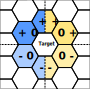
\includegraphics{graphics/scatter.png}
    \caption{Scattering without a scatter die.}
    \label{fig:scatter-alternative}
\end{figure}